\documentclass[12pt]{article}
\usepackage[utf8]{inputenc}
\usepackage{array}
\usepackage{amsthm}
\usepackage{amsmath}
\usepackage{amsfonts}
\usepackage{amssymb}
\usepackage{mathtools}
\usepackage{tikz}
\usepackage{graphicx}
\usepackage{caption}
\usepackage{subcaption}
\usepackage{hyperref}
\usepackage{float}
\usepackage{blindtext}
\usepackage{titlesec}
\usepackage[legalpaper, margin=1.2in]{geometry}
%\usepackage{setspace} \doublespacing

\graphicspath{ {./graphs/} }

\title{STA 2503/MMF 1928 Project 2 - Delta-Gamma Hedging}
\author{Dixin Mou, Juliano Zhu, Wenhao Li}
\date{2022/11/13}

\begin{document}
\begin{titlepage}
  \begin{center}
      \vspace*{7cm}

      \textbf{STA 2503/MMF 1928 Project 2 - Delta-Gaama Hedging}

      % \vspace{0.5cm}
      %  Thesis Subtitle
           
      \vspace{1.5cm}

      \textbf{Dixin Mou, Juliano Zhu, Wenhao Li}

      \vfill
           
      % A thesis presented for the degree of\\
      % Doctor of Philosophy
           
      \vspace{0.8cm}
           
      % Department Name\\
      University of Toronto\\
      Toronto, Ontario, Canada\\
      November $13^{th}$, 2022 
           
  \end{center}
\end{titlepage}


\section{Abstract}
The option is one of the risky financial derivatives. Trader who long or short the options always need to manage its risk. The most strategy that used is dynamic hedging, which requires constant position and portfolio adjustment. By mathematical 
derivation and programming simulation, this project provides the frameworks and implement details of delta and delta-gamma hedging strategies with time-based and moved-based hedging approaches on different bands. The final report explains the 
differences between the two hedging strategies with two different approaches by the distributions of position and portfolio value change, profit/loss analyses and the efficient frontier analyses with different transaction costs.

\newpage
\tableofcontents

\newpage
\listoffigures

\newpage
\section{Introduction}
This project focuses on the implementation of the delta and gamma dynamic hedging with time-based and move-based hedging strategy. Compared with delta-hedging, delta-gamma hedging is more sophisticated dynamic hedging with eliminating more risk. 
Move-based hedging has easier operations but with more times of transactions. The project studies the differences between delta-hedging and delta-gamma-hedging with combination of time-based or moved-based hedging strategies.


\section{Model Setup}
In this project, an at-the-money $\frac{1}{4}$ year put written on the underlying asset is shorted and the aim is to hedge it. The transaction cost is considered: equity transaction cost is \$0.005 per unit and option transaction cost is \$0.01 per unit.\\
\\Suppose that the European call and put option with underlying asset $S=(S_{t_k})_{k \in (0,1,...,N)}$, $S_{t_0}$ = \$100 are given and satisfies the Black-Scholes Model. Therefore, their prices are given by the Black-Scholes formulas for the prices of European call (C) and put (P) options:
\begin{equation}
    C({S_{t_k}},{t_k}) = {S_{t_k}} {\Phi(d_+)} - K {e^{-r(T-{t_k})}} {\Phi(d_-)}
\end{equation}
\begin{equation}
    P({S_{t_k}},{t_k}) = K {e^{-r(T-{t_k})}} {\Phi(-d_-)} - {S_{t_k}} {\Phi(-d_+)}
\end{equation}
where
\begin{equation}
    {d_+} = \frac{ln({\frac{{S_{t_k}}}{K}}) + (r+{\frac{1}{2}}{\sigma^2})(T-{t_k})}   
    {{\sigma}{\sqrt{T-{t_k}}}}
\end{equation}
\begin{equation}
    {d_+} = \frac{ln({\frac{{S_{t_k}}}{K}}) + (r-{\frac{1}{2}}{\sigma^2})(T-{t_k})}   
    {{\sigma}{\sqrt{T-{t_k}}}}
    ~~
    ={d_+} - {{\sigma}{\sqrt{T-{t_k}}}}
\end{equation}
K is the strike price, which is set equal to \$100 for both European put and call option.\\
\\T is the maturity date. For the following methodology and strategy, the maturity of the put option is 90 days, which is a quarter of a year (360 days). And the maturity of the call option is 180 days, which is half of a year.\\
\\${t_k}$ is the time and ${\Delta}$t is the time step, which is set to be a daily basis, k $\in$ [0,1,...,90].\\
${\Delta}$t = 1 day. $t_0=0$ is the initial time and $t_n$ is the maturity, n=90;\\
\\r is the continuous risk-free rate, which is equal to 0.02.\\
\\$\sigma$ is the volatility rate, which is equal to 0.2.\\
\\${\Phi(d_-)}$ $\in$ [0,1] is the probability that a call option will be exercised in a risk-neutral world.\\
\\${\Phi(d_+)}$ $\in$ [0,1] does not have a fairly simple interpretation like ${\Phi(d_-)}$. But it's use can interpreted and comprehended in another way:\\
\\In a risk-neutral world, for a call option, 
${S_{t_0}}{\Phi(d_+)}{e^{rT}}$ is the expected stock price at time T when stock prices less than the strike price are counted as zero. The strike price K is only paid if the stock price is greater than K and this has a probability of ${\Phi(d_-)}$. The expected payoff is ${S_{t_0}}{\Phi(d_+)}{e^{rT}} - K{\Phi(d_-)}$. Discounting this to time 0 gives the Black–Scholes equation for a European call option:
\begin{equation}
    C({S_{t_0}},{t_0}) = {S_{t_0}} {\Phi(d_+)} - K {e^{-rT}} {\Phi(d_-)}
\end{equation}
And according to the put-call parity equation,
\begin{equation}
    C({S_{t_0}},{t_0}) - P({S_{t_0}},{t_0}) = {S_{t_0}} - {K{e^{-eT}}}
\end{equation}
It gives the equation for European put option:
\begin{equation}
    P({S_{t_0}},{t_0}) = K {e^{-rT}} {\Phi(-d_-)} - {S_{t_0}} {\Phi(-d_+)}
\end{equation}
To simulate the case in real life, 10000 paths are run by the programming approach.




\section{Methodology}

\subsection{Delta}
The term delta of an option refers to the rate of change of the option price (f) with respect to the change of the underlying asset price (S). It represents the first order risk measure that indicates how sensitive a derivative is to the changes in the underlying asset price, while all other variables remain unchanged. It’s also the slope of the curve (at a point) of the option price to the underlying asset price. 
\begin{equation}
    {\Delta} = {\frac{{\partial f}}{{\partial S}}}
\end{equation}
For the European call (C) and put (P), the deltas are:
\begin{equation}
    {\Delta^{Call}} = {\frac{{\partial C}}{{\partial S}}} = \Phi(d_+)
\end{equation}
\begin{equation}
    {\Delta^{Put}} = {\frac{{\partial P}}{{\partial S}}} = \Phi(d_+)-1
\end{equation}
where
${\Phi(d_+)}$ $\in$ [0,1], so ${\Delta^{Call}}$ $\in$ [0,1] and ${\Delta^{Put}}$ $\in$ [-1,0]. This indicates call option price and put option price has a positive and negative correlation with underlying asset price respectively.

\subsection{Gamma}
The term gamma of an options refer to the rate of change of the option’s delta ($\Delta$) with respect to the change of the underlying asset price (S).  It’s the second partial derivative of the option price (f) with respect to the underlying asset price (S).\\
\\For the European call (C) and put (P), the gammas are:
\begin{equation}
    {\Gamma^{Call}} = {\frac {\partial^2 C} {\partial S^2}} = {\frac {\partial \Delta^{Call}} {\partial C}} = {\Gamma^{Put}}
\end{equation}

\subsection{Delta Hedging Strategy}
Delta hedging is a trading strategy that aims to reduce, or hedge, the directional risk associated with price movements in the underlying asset. The most basic type of delta hedging involves an investor who buys or sells options and then offsets the delta risk by bank account and buying or selling a certain amount of underlying assets. Investors may want to offset their risk of moving in the option or the underlying stock by using delta hedging strategies and reach a delta-neutral state without a directional bias on the hedge. Since delta hedging attempts to neutralize or reduce the extent of the move in an option's price relative to the asset's price, it requires a constant rebalancing of the hedge. In other words, the dynamic hedging portfolio is a delta-neutral portfolio whose value is unaffected by (first-order) changes in the value of the underlying asset S.\\
\\Mathematically, to implement the dynamic delta hedging, the model includes:\\
(1) A source of uncertainty given by the Itô's process $S=(S_{t_k})_{k \geq 0}$ satisfying the SDE:
\begin{equation}
    {\frac{dS_{t_k}}{S_{t_k}}} = {\mu^S_{t_k}} {dt} + {\sigma^S_{t_k}}{dW_{t_k}}
\end{equation}
where\\
\\${\mu^S_{t_k}}$ is the stock drift rate, which is equal to 0.1;\\
\\${\sigma^S_{t_k}}$ is the stock volatility rate, which is equal to 0.2;\\
\\${W_{t_k}}$ is the brownian motion, ${W_{t_k}}$ $\sim$ N(0,t).\\
\\For the project, the underlying asset is the source of uncertainty.\\
\\(2) A bank account (process), $B=(B_{t_k})_{k \geq 0}$, satisfying the SDE:
\begin{equation}
    {\frac{dB_{t_k}}{B_{t_k}}} = {r_{t_k}}{dt}
\end{equation}
where ${r_{t_k}}=0.02$\\
\\(3) A traded claim written on the source of uncertainty whose price price process, $f=(f_{t_k})_{k \geq 0}$, satisfying the SDE:
\begin{equation}
    {\frac{df_{t_k}}{f_{t_k}}} = {\mu^f_{t_k}} {dt} + {\sigma^f_{t_k}}{dW_{t_k}}
\end{equation}
(4) A second contingent claim written on S, whose price process denoted as $g=(g_{t_k})_{k \geq 0}$, and g(T,$S_{t_n}$)=G($S_{t_n}$). g also satisfies the SDE:
\begin{equation}
    {\frac{dg_{t_k}}{g_{t_k}}} = {\mu^g_{t_k}} {dt} + {\sigma^g_{t_k}}{dW_{t_k}}
\end{equation}
Then to construct the delta-neutral portfolio, the portfolio should be zero cost and self-financing with investing (${\alpha}$,${\beta}$)=(${\alpha}_{t_k}$,${\beta}_{t_k}$)$_{k \geq 0}$ unit for f and B respectively and shorting one unit of g. The portfolio is:
\begin{equation}
    {V_{t_k}} = {{\alpha}_{t_k}} {f_{t_k}} + {{\beta}_{t_k}} {B_{t_k}} - {g_{t_k}}
\end{equation}
In terms of SDE, the dynamic portfolio value is:
\begin{equation}
    {dV_{t_k}} = ({{\alpha}_{t_k}} {f_{t_k}} {\mu^f_{t_k}} + {{\beta}_{t_k}} {B_{t_k}} {r_{t_k}} - {g_{t_k}}{\mu^g_{t_k}})dt + ({{\alpha}_{t_k}} {f_{t_k}} {\sigma^f_{t_k}} - {g_{t_k}}{\sigma^g_{t_k}}){dW_{t_k}}
\end{equation}
Since the portfolio is risk-free, the instantaneous risk need to be removed. The coefficient of $dW_{t_k}$ is set to be zero:
\begin{equation}
    {\alpha^*_{t_k}} {f_{t_k}} {\sigma^f_{t_k}} - {g_{t_k}} {\sigma^g_{t_k}}=0
\end{equation}
\begin{equation}
    {\alpha^*_{t_k}} = {\frac{ {g_{t_k}} {\sigma^g_{t_k}} }  { {f_{t_k}} {\sigma^f_{t_k}} } }
\end{equation}
In the project, the underlying asset stock is traded and is used to be an hedging instrument, so ${f_{t_k}} = {S_{t_k}}$. And the at-the-money put option (${P_{t_k}}$) that shorted is the second contingent claim (${g_{t_k}}$) written on S.
\begin{equation}
    \longrightarrow {\alpha^*_{t_k}} = {\frac{ {P_{t_k}} {\sigma^P_{t_k}} }  { {S_{t_k}} {\sigma^S_{t_k}} } } 
    ~~ and ~~
    {V_{t_k}} = {{\alpha}_{t_k}} {S_{t_k}} + {{\beta}_{t_k}} {B_{t_k}} - {P_{t_k}}
\end{equation}
In addition,
\begin{equation}
    {\frac{dg_{t_k}}{g_{t_k}}} = {\mu^g_{t_k}} {dt} + {\sigma^g_{t_k}}{dW_{t_k}}
    ~~ \to ~~
    {dg_{t_k}} = {g_{t_k}}{\mu^g_{t_k}} {dt} + {g_{t_k}}{\sigma^g_{t_k}}{dW_{t_k}}
\end{equation}
Itô's Lemma:
\begin{equation}
    {g_{t_k}} = ({\delta_t}{g_{t_k}} + {\mu^S_{t_k}} {S_{t_k}} \cdot {\delta_S}{g_{t_k}} + {\frac{1}{2}} {{\sigma^S_{t_k}}^2} {{S_{t_k}}^2}  \cdot  {\delta_{SS}}{g_{t_k}})dt 
    + ( {\sigma^S_{t_k}} {S_{t_k}} \cdot {{\delta}_{S}}{g_{t_k}} ){dW_{t_k}}
\end{equation}
Equations (14) \& (15) give:
\begin{equation}
    {g_{t_k}}{\sigma^g_{t_k}} = {\sigma^S_{t_k}} {S_{t_k}} \cdot {{\delta}_{S}}{g_{t_k}}
    ~~ \to ~~
    {P_{t_k}}{\sigma^P_{t_k}} = {\sigma^S_{t_k}} {S_{t_k}} \cdot {{\delta}_{S}}{P_{t_k}}
\end{equation}
\begin{equation}
    \to  {\alpha^*_{t_k}} = {\frac{ {\sigma^S_{t_k}} {S_{t_k}} \cdot {{\delta}_{S}}{P_{t_k}} }  
    { {S_{t_k}} {\sigma^S_{t_k}} } } = {{\delta}_{S}}{P_{t_k}}
\end{equation}
which is the delta of the put option ${\Delta^{Put}_{t_k}}$ \\
\\Then the portfolio has:
\begin{equation}
    {V_{t_k}} = {\alpha^*_{t_k}} {S_{t_k}} + {{\beta}_{t_k}} {B_{t_k}} - {P_{t_k}}
\end{equation}
\begin{equation}
    \longrightarrow {\Delta^{V}_{t_k}} = {\alpha^*_{t_k}} {\Delta^{S}_{t_k}} + {{\beta}_{t_k}}{\Delta^{B}_{t_k}} - {\Delta^{Put}_{t_k}}
\end{equation}
where
\begin{equation}
    {\Delta^{S}_{t_k}} = {\frac{dS}{dS}} = 1
    ~~ and ~~
    {\Delta^{B}_{t_k}} = {\frac{dB}{dS}} = 0
\end{equation}
\begin{equation}
    \longrightarrow {\Delta^{V}_{t_k}} = {\Delta^{Put}_{t_k}} \cdot 1 + 0 - {\Delta^{Put}_{t_k}} = 0
\end{equation}
\begin{equation}
    \longrightarrow {V_{t_k}} = {\alpha^*_{t_k}} {S_{t_k}} + {{\beta}_{t_k}} {B_{t_k}} - {P_{t_k}} = 0
\end{equation}
which indicates the portfolio is delta-neutral.\\
\\In summary, in the delta-hedging strategy, the portfolio is constructed by shorting an at-the-money put option and longing ${\alpha_{t_0}}$ units stocks at the beginning. And then the hedging portfolio is rebalanced to keep being delta-neutral by the bank account and adjusting the position (${\alpha_{t_k}}$) of the underlying stock at each time step to hedge the short position risk of the put option as time goes forward and price changes. In other words, the portfolio should be kept with zero net delta.\\
\\The table below explains the detail of rebalancing transactions and the value of put option and bank account, at each time step:\\
\\ $\phi_1$ is the equity transaction cost, $\phi_1$ = \$0.005;\\
\\For bank account, if at some time steps, the bank account has negative value, the cash is borrowed to long units of stock S. Otherwise, the cash is placed from the short sale of the stock S into the bank account B. And the long or short of stock S is financed by borrowing or lending from bank account.

\begin{enumerate}
  \item $t=0$ day
  \begin{itemize}
    \item Short a put option with price $P_0=P(t_0, S_0)$
    \item Long $\alpha_0=\Delta^{put}(0, S_0)$ of stock at stock price $S_0$, cost $\alpha_0S_0 + |\alpha_0|\phi_1$
    \item After transactions above, bankaccount contains $B_0=P_0-\alpha_0S_0 - |\alpha_0|\phi_1$
  \end{itemize}

  \item $t=1$ day
  \begin{itemize}
    \item $S_0 \rightarrow S_1$
    \item rebalance: $\alpha_0 \rightarrow \alpha_1$, $\alpha_1 = \Delta^{put}(1, S_1)$
    \item $B_0 \rightarrow B_0e^{r\Delta t}$, $B_1 = B_0e^{r\Delta t} - (\alpha_1-\alpha_0)S_0 - |\alpha_1-\alpha_0|\phi_1$
  \end{itemize}
  
  \item $t=k$ day
  \begin{itemize}
    \item $S_{k-1} \rightarrow S_k$
    \item rebalance: $\alpha_{k-1} \rightarrow \alpha_k$, $\alpha_k = \Delta^{put}(k, S_k)$
    \item $B_k \rightarrow B_{k-1}e^{r\Delta t}$, $B_k = B_{k-1}e^{r\Delta t} - (\alpha_k-\alpha_{k-1})S_0 - |\alpha_k-\alpha_{k-1}|\phi_1$
  \end{itemize}

  \item $t=N$ day
  \begin{itemize}
    \item $S_{N-1} \rightarrow S_N$
    \item Pay potential put option payoff, $G = max(K-S_N,0)$
    \item $B_N \rightarrow B_{N-1}e^{r\Delta t}$, use financial settlement:\\
      $B_N = B_{N-1}e^{r\Delta t} + \alpha_{N-1}S_N + |\alpha_{N-1}|\phi_1 -G$
  \end{itemize}
\end{enumerate}

\subsection{Delta-Gamma Hedging Strategy}
Another more sophisticated dynamic hedging strategy is delta-gamma hedging strategy. As indicated by the delta and gamma equations above, delta refers to a change in the price of an option contract per change in the price of the underlying asset and gamma refers to the rate of change of delta.\\
\\The delta-gamma hedging combines both delta and gamma hedges to mitigate the risk of changes in the underlying asset S and in the delta itself. This means, in addition to the elimination of the risk that delta hedged, delta-gamma hedging reduces the risk associated with changes in an option's delta. This is the basis for delta-gamma-hedging which could protect the portfolio against both small and large price changes between rebalancing. Delta-gamma hedging also measures the slope of the curve (at a point) of the option price to the underlying asset price using a quadratic function instead of a straight line. \\
\\Similar to the delta hedging which aims to keep the portfolio delta-neutral by rebalancing dynamically, the delta-gamma hedging aims to keep the portfolio delta-gamma-neutral by rebalancing dynamically.\\
\\To implement the delata-gamma hedging, in addition to the underlying asset S, bank account B, a traded claim f (in project case is S) and a second contingent claim g written on S (in project case is the at-the-money put option P that shorted), a hedging option with value h($t_k$,$S_{t_k}$) and h(T,$S_{t_n}$) = H($S_{t_n}$) needs to be introduced. It also satisfies the SDE:
\begin{equation}
    {\frac{dh_{t_k}}{h_{t_k}}} = {\mu^h_{t_k}} {dt} + {\sigma^h_{t_k}}{dW_{t_k}}
\end{equation}
Then, to construct the delta-gamma-neutral portfolio, one needs to construct the portfolio to be zero cost and self-financing with investing (${\alpha}$,${\beta}$,${\eta}$)=(${\alpha}_{t_k}$,${\beta}_{t_k}$,${\eta}_{t_k}$)$_{k \geq 0}$ unit for f, B, h respectively and shorting one unit of g. The portfolio is:
\begin{equation}
    {V_{t_k}} = {{\alpha}_{t_k}} {f_{t_k}} + {{\beta}_{t_k}} {B_{t_k}} +{\eta}_{t_k}{h_{t_k}} - {g_{t_k}}
\end{equation}
In the project, ${f_{t_k}} = {S_{t_k}}$, ${g_{t_k}} = {P_{t_k}}$ and the hedging option h that introduced is a call option C with maturity $\frac{1}{4}$ year and strike price \$100.
\begin{equation}
    \longrightarrow {V_{t_k}} = {{\alpha}_{t_k}} {S_{t_k}} + {{\beta}_{t_k}} {B_{t_k}} +{\eta}_{t_k}{C_{t_k}} - {P_{t_k}}
\end{equation}
The delta of the portfolio is:
\begin{equation}
    {\Delta^{V}_{t_k}} = {\alpha_{t_k}} + {{\eta}_{t_k}}{\Delta^{Call}_{t_k}} - {\Delta^{Put}_{t_k}}
\end{equation}
The gamma of the portfolio is:
\begin{equation}
    {\Gamma^{V}_{t_k}} = {{\eta}_{t_k}}{\Gamma^{Call}_{t_k}} - {\Gamma^{Put}_{t_k}}
\end{equation}
The delta-gamma-neutral asks delta and gamma of the portfolio to be zero:
\begin{equation}
    {\Delta^{V}_{t_k}} = 0 
    ~~ and ~~ 
    {\Gamma^{V}_{t_k}} = 0
\end{equation}
\begin{equation}
    \longrightarrow {\alpha^*_{t_k}} = -{{\eta}_{t_k}}{\Delta^{Call}_{t_k}} + {\Delta^{Put}_{t_k}}
    ~~ and ~~ 
    {{\eta}^*_{t_k}} = \frac{\Gamma^{Put}_{t_k}}{\Gamma^{Call}_{t_k}}
\end{equation}
which gives the required number of units need to be held in the underlying asset S and the hedging option C.\\
\\And,
\begin{equation}
    {V_{t_k}} = 0
\end{equation}
In summary, in the delta-gamma-hedging strategy, the portfolio is constructed by shorting an at-the-money put option, longing ${\alpha_{t_0}}$ units stocks and longing ${\eta_{t_0}}$ units European call option at the beginning. And then the hedging portfolio is rebalanced to keep being delta-gamma-neutral by the bank account and adjusting the position ${\alpha_{t_k}}$ of the underlying stock and the position ${\eta_{t_k}}$ of the call option at each time step to hedge the short position risk of the put option as time goes forward and price changes. In other words, the portfolio should be kept with zero net delta and zero net gamma.\\
\\The table below explains the detail of rebalancing transactions and the value of put option and bank account, at each time step:\\
\\ $\phi_1$ is the equity transaction cost, $\phi_1$ = \$0.005;\\
\\ $\phi_2$ is the option transaction cost, $\phi_2$ = \$0.01;\\
\begin{enumerate}
  \item $t=0$ day
  \begin{itemize}
    \item Short a put option with price $P_0=P(t_0, S_0)$
    \item Long $\gamma_0 = \frac{\Gamma^{put}_0}{\Gamma^{call}_0}$ of call option, cost $\gamma_0C_0 + |\gamma_0|\phi_2$
    \item Long $\alpha_0 = \Delta^{put}_0-\frac{\Gamma^{put}_0}{\Gamma^{call}_0}\Delta^{call}_0$ of stock at stock price $S_0$, cost $\alpha_0S_0 + |\alpha_0|\phi_1$
    \item After transactions above, bankaccount contains:\\
       $B_0=P_0-\alpha_0S_0 - |\alpha_0|\phi_1 - \gamma_0C_0 + |\gamma_0|\phi_2$
  \end{itemize}

  \item $t=1$ day
  \begin{itemize}
    \item $S_0 \rightarrow S_1$
    \item rebalance call option position: $\gamma_0 \rightarrow \gamma_1$, $\gamma_1 = \frac{\Gamma^{put}_1}{\Gamma^{call}_1}$
    \item rebalance stock position: $\alpha_0 \rightarrow \alpha_1$, $\alpha_1 = \Delta^{put}_1-\frac{\Gamma^{put}_1}{\Gamma^{call}_1}\Delta^{call}_1$
    \item $B_0 \rightarrow B_0e^{r\Delta t}$, $B_1 = B_0e^{r\Delta t} - (\alpha_1-\alpha_0)S_1 - |\alpha_1-\alpha_0|\phi_1 - (\gamma_1-\gamma_0)C_1 - |\gamma_1-\gamma_0| \phi_2$
  \end{itemize}
  
  \item $t=k$ day
  \begin{itemize}
    \item $S_{k-1} \rightarrow S_k$
    \item rebalance call option position: $\gamma_{k-1} \rightarrow \gamma_k$, $\gamma_k = \frac{\Gamma^{put}_k}{\Gamma^{call}_k}$
    \item rebalance stock position: $\alpha_{k-1} \rightarrow \alpha_k$, $\alpha_k = \Delta^{put}_k-\frac{\Gamma^{put}_k}{\Gamma^{call}_k}\Delta^{call}_k$
    \item $B_{k-1} \rightarrow B_ke^{r\Delta t}$:\\\\
     $B_k = B_{k-1}e^{r\Delta t} - (\alpha_k-\alpha_{k-1})S_k - |\alpha_1-\alpha_{k-1}|\phi_1 - (\gamma_k-\gamma_{k-1})C_k - |\gamma_k-\gamma_{k-1}| \phi_2$
  \end{itemize}

  \item $t=N$ day
  \begin{itemize}
    \item $S_{N-1} \rightarrow S_N$
    \item Pay potential put option payoff, $G = max(K-S_N,0)$
    \item $B_N \rightarrow B_{N-1}e^{r\Delta t}$, use financial settlement:\\
      $B_N = B_{N-1}e^{r\Delta t} + \alpha_{N-1}S_N + |\alpha_{N-1}|\phi_1 + \gamma_{N-1}S_N + |\gamma_{N-1}|\phi_2 - G$
  \end{itemize}
\end{enumerate}

\subsection{Time-based Hedging Strategy}
Time-based hedging requires position adjustment at each time step increment. The length of the time step and the number of time steps are set in advance.\\
\\For the delta hedging, the strategy starts at ${\alpha_{t_0}}$ units stocks at time 0. After one time step, it re-hedges with new unit ${\alpha_{t_1}}$ of the underlying asset and amount of bank account. In general, at time step ${t_k}$, time-based hedging strategy re-hedges and rebalances the portfolio like the transaction operations that the table above explained. The delta-gamma hedging works in a similar way except the unit of hedging option also needs adjustment.\\
 

\subsection{Move-based Hedging Strategy}
Move-based hedging strategy does not rebalance the portfolio at each time step but at the time when the value of underlying asset position hit the band that set.\\
\\For the delta hedging, the strategy starts at ${\alpha_{t_0}}$ units stocks at time 0 and place a band right around ${\alpha_{t_0}}$ equally and symmetrically. Then the value of ${\alpha_{t_k}}$ is followed as time goes forward and underlying asset price changes. The ${\alpha_{t_k}}$ will not be changed until the value of it hit the band. Once the ${\alpha_{t_k}}$ hit the band, whether the upper band or the lower band, the portfolio will be re-hedged and rebalanced, and also a new band will be placed symmetrically around the new position ${\alpha_{t_k}}$. The delta-gamma hedging works in a similar way except the unit of hedging option also needs adjustment.\\
\\The time that the portfolio is re-hedged and rebalanced depends on when the position of the underlying asset hit the band around the current position. As a result, unlike the time-based hedging, the number of re-hedging and rebalancing is random. It depends on the actual outcome of the underlying asset price.\\
\\Move-based hedging strategy require continuous monitoring of the underlying asset price. But compared to the time-based hedging strategy, it requires less adjustment to the delta and gamma position parameters if the position keeps within the bound range.\\
\\In the project, the band width is 0.1, the upper bound is -0.01 and the lower bound is -0.99.




\section{Result}
To perform a more intuitive illustration, hedging position plots are based on 10 simulation paths. And the number of trade plots are based on 10000 simulation paths. Both time-based and move-based portfolios converged to either 0 or -1 at maturity, since from the formula above, 
the derivative of the option price will approach 0 and -1.
\begin{figure}[H]
  \centering
  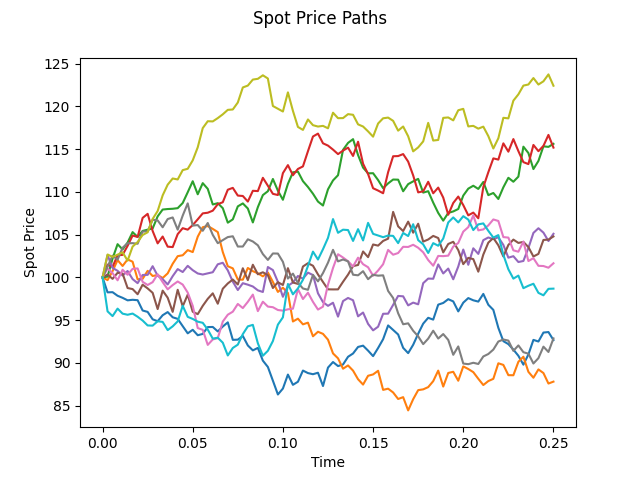
\includegraphics[scale=0.8]{price.png}
  \caption{Simulated Examples of Stock Price Process}
\end{figure}
\subsection{Delta Hedging}
\begin{figure}[H]
  \centering
  \begin{subfigure}{.5\textwidth}
    \centering
    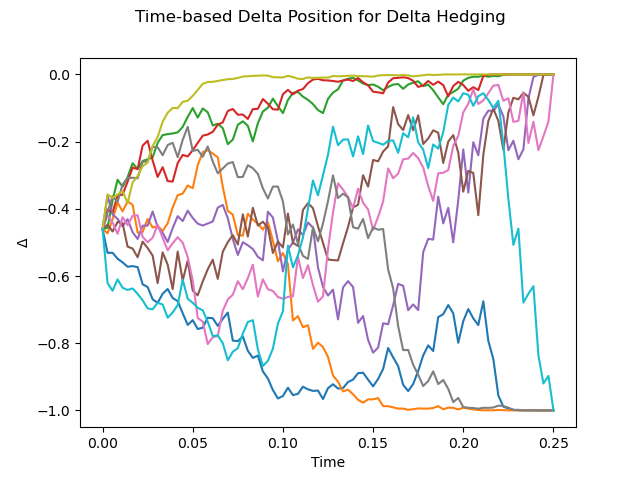
\includegraphics[width=\linewidth]{position-delta-time.png}
    \caption{Time-based}
  \end{subfigure}%
  \begin{subfigure}{.5\textwidth}
    \centering
    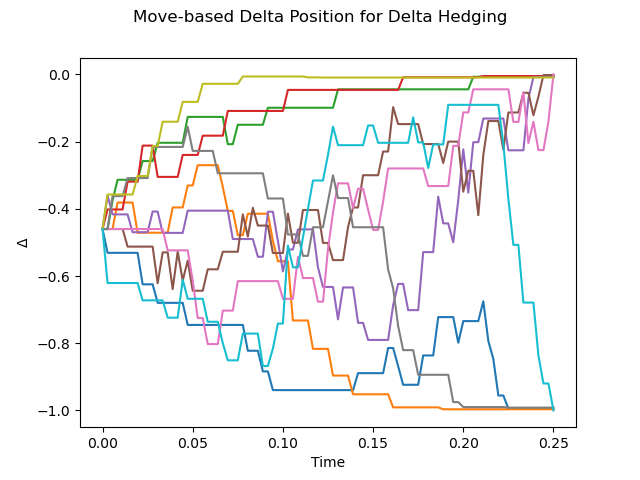
\includegraphics[width=\linewidth]{position-delta-move.png}
    \caption{Move-based}
  \end{subfigure}%
  \caption{Position of Spot Hold for Delta Hedging}
\end{figure}

It can be clearly observed that the movement of the price path is similar to the position path. For example, the orange colour path increased to 105 at time 0.06 then started to decrease all the way to the end. The hedging position follows the same pattern: the short position 
increased from $-0.2$ at time $0.06$ to $-1$ at maturity. It also can be explained it from a financial perspective: since the stock price has a decreasing trend, to hedge a great amount of payoff payment at exercise time, the portfolio should obtain a more short position in the stock
 and realize the gain from the price decrease to offset the payoff payment. By the same logic, the bank account value is the inverse version of the hedging position.
\\\\
Time-based and move-based position paths are quite similar to each other. The move-based portfolio will not adjust the position until the delta breaks the band boundary - returning a piecewise function. The trade time can be considered random but determined by delta. The 
time-based portfolio adjusts the position at each time increment, the smaller the delta-t, the more frequent adjustment will be. Since the portfolio includes the transaction cost into consideration, it will also make the time-based strategy to be costlier and more wasteful, 
especially during the convergence period which the position does not change much(for example the yellow, green and red paths from $t = 0.125$ to $0.25$). The move-based strategy did a great job in this situation, the green and red paths were much less frequently adjusted.
\\\\
It is also reflected in the number of trade plots shown below. The means of the two distributions are 3.5 and 2.5 respectively.

\begin{figure}[H]
  \centering
  \begin{subfigure}{.5\textwidth}
    \centering
    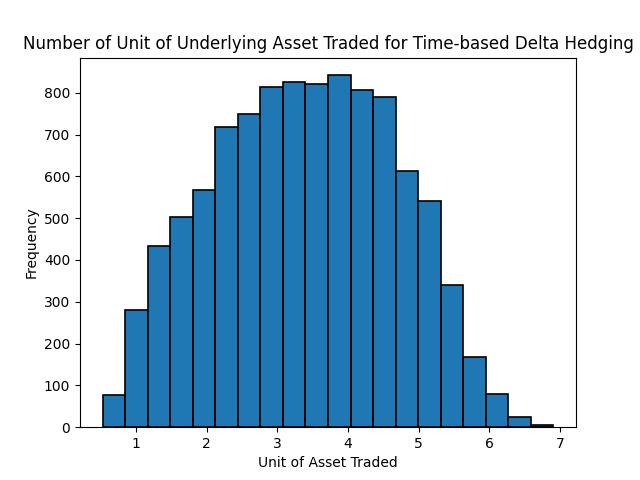
\includegraphics[width=\linewidth]{num-trade-time.png}
    \caption{Time-based}
  \end{subfigure}%
  \begin{subfigure}{.5\textwidth}
    \centering
    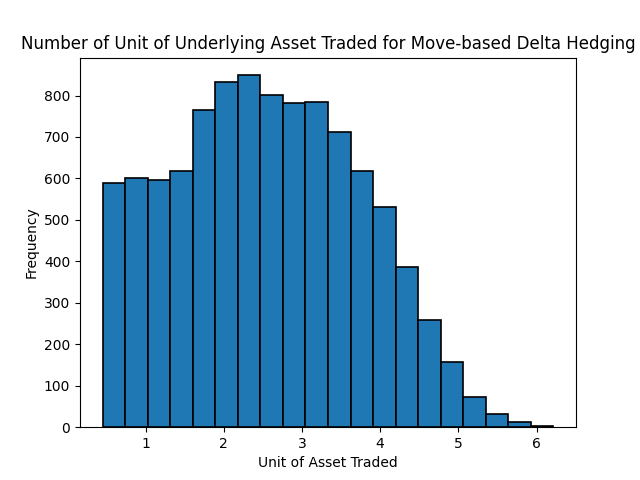
\includegraphics[width=\linewidth]{num-trade-move.png}
    \caption{Move-based}
  \end{subfigure}%
  \caption{Number of Total Stock Transactions During Delta Hedging}
\end{figure}

\subsubsection{Profit \& Loss Analysis}
\begin{figure}[H]
  \centering
  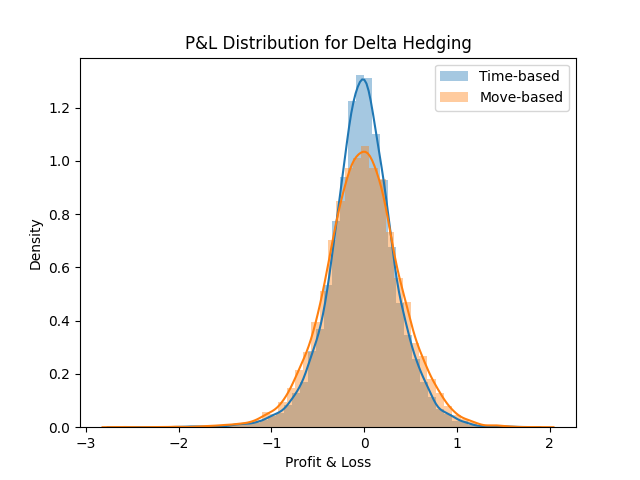
\includegraphics[scale=0.8]{PnLDistributionforDeltaHedging.png}
  \caption{P\&L Distribution for Delta Hedging}
\end{figure}

To perform a more intuitive illustration, P\&L distributions are based on 10000 simulation paths. 
For the profit and loss distribution diagram, the mean of both portfolios is very close to zero which matches the delta-neutral dynamic hedging portfolio assumption. The move-based method has a distribution with greater variance($0.13002<0.17269$) and a fatter tail than the time-based method. 
The expected return is slightly greater than the time-based portfolio ($-0.018951 < -0.016592$). It’s also reasonable in the real-life financial market that a larger variance portfolio usually comes with a larger mean return.

\subsubsection{Conditional Value at Risk Analysis}
To perform a more intuitive illustration, P\&L distributions with VaR and CVaR are based on 10000 simulation paths. 
To find the put option price that makes the profit and loss conditional value-at-risk at level 0.90 no larger than 0.02, the team decided to find the value difference between the conditional value-at-risk(loss) at the 0.1 percentile and benchmark conditional value-at-risk value. 
Then the adjustment amount of the put option price will be the present value of the difference.

\begin{figure}[H]
  \centering
  \begin{subfigure}{.5\textwidth}
    \centering
    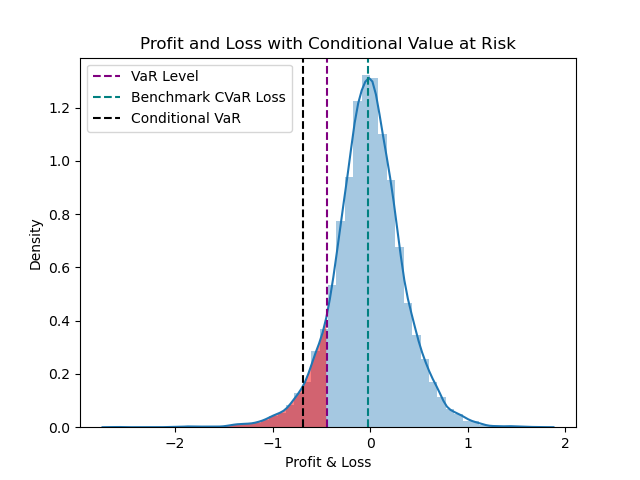
\includegraphics[width=\linewidth]{delta-var-t.png}
    \caption{Time-based}
  \end{subfigure}%
  \begin{subfigure}{.5\textwidth}
    \centering
    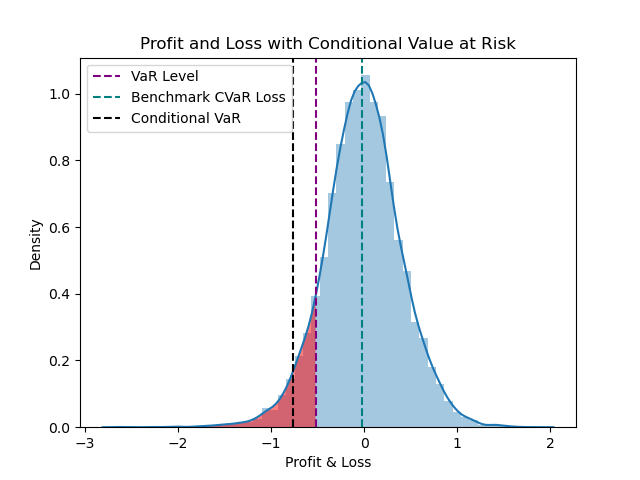
\includegraphics[width=\linewidth]{delta-var-m.png}
    \caption{Move-based}
  \end{subfigure}%
  \caption{P\&L with Conditional Value at Risk for Delta Hedging}
  %\label{fig:test}
\end{figure}

The following shows the CVaR and adjusted option price observed: 
\begin{enumerate}

  \item The unadjusted option price according to the Delta hedging is 3.7334
  \item CVaR-adjusted option price for Time-based hedging portfolio:

  \begin{itemize}

    \item The VaR for the portfolio at level 0.1 is -0.4459
    \item The CVaR for the portfolio at VaR level 0.1 is -0.6837
    \item The Adjusted put option price so CVaR at VaR level 0.1 is no smaller than -0.02 is 4.3938

  \end{itemize}

  \item CVaR-adjusted option price for Move-based hedging portfolio:
  
  \begin{itemize}

    \item The VaR for the portfolio at level 0.1 is -0.5212
    \item The CVaR for the portfolio at VaR level 0.1 is -0.7679
    \item The Adjusted put option price so CVaR at VaR level 0.1 is no smaller than -0.02 is 4.4776

  \end{itemize}

\end{enumerate}

\noindent
The move-based portfolio P\&L has both larger VaR and CVaR than the time-based portfolio, it matches the conclusion made in part one: the move-based portfolio has a greater variance and fatter tail. It brings extreme cases (extreme loss and gain) which will be greater than the 
time-based portfolio. Therefore, it requires charging a larger option price to make sure the loss is kept in the optimal range.

\subsection{Delta-Gamma Hedging}
To perform a more intuitive illustration, hedging position plots are based on 10 simulation paths. And P\&L distributions are based on 10000 simulation paths. 
\\\\
The time and move basis of delta and delta-gamma hedging strategies follow the same logic. In the delta-gamma hedging strategy, the underlying asset position plot seems to be inverse to the call option position plot. For example, the yellow-green path, when the stock price increase, 
the portfolio would short fewer assets (i.e. prevent loss from price raise) and long more call options (i.e. gain positive payoff at the exercise date if the price keeps increasing).

\begin{figure}[H]
  \centering
  \begin{subfigure}{.5\textwidth}
    \centering
    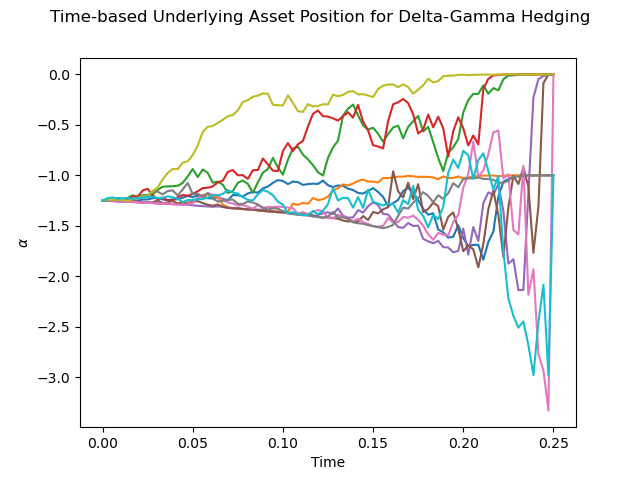
\includegraphics[width=\linewidth]{asset-time.png}
    \caption{Time-based}
  \end{subfigure}%
  \begin{subfigure}{.5\textwidth}
    \centering
    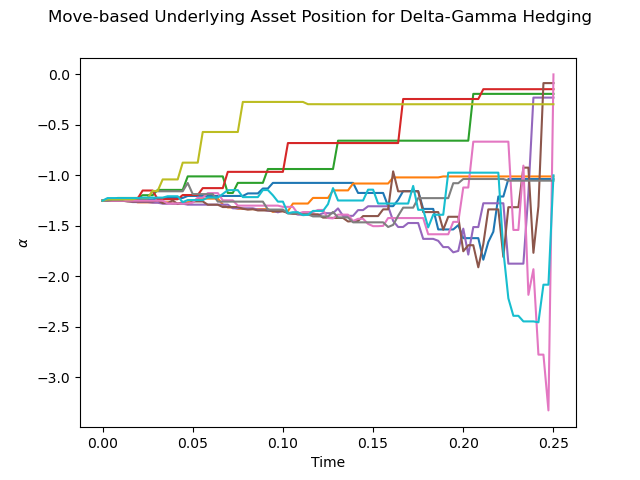
\includegraphics[width=\linewidth]{asset-move.png}
    \caption{Move-based}
  \end{subfigure}%
  \caption{Position of Spot Hold for Delta-Gamma Hedging}
\end{figure}

\begin{figure}[H]
  \centering
  \begin{subfigure}{.5\textwidth}
    \centering
    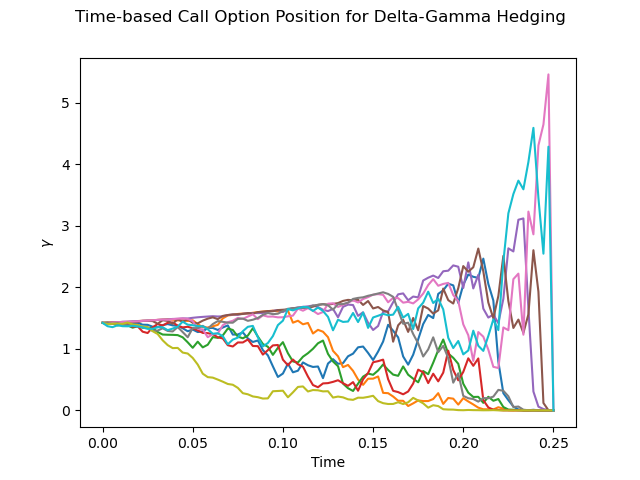
\includegraphics[width=\linewidth]{call-time.png}
    \caption{Time-based}
  \end{subfigure}%
  \begin{subfigure}{.5\textwidth}
    \centering
    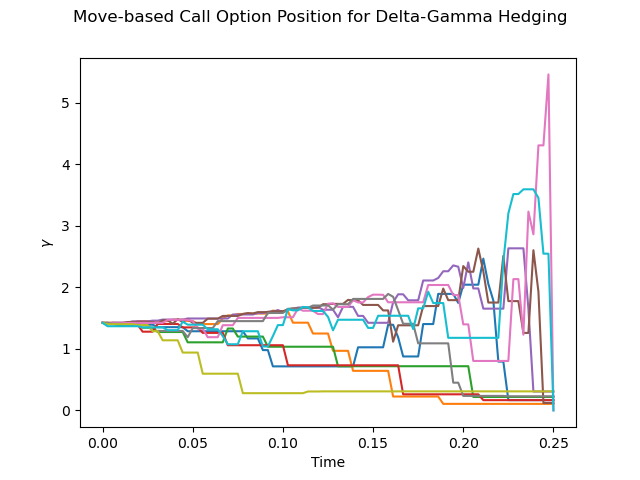
\includegraphics[width=\linewidth]{call-move.png}
    \caption{Move-based}
  \end{subfigure}%
  \caption{Position of Call Option Hold for Delta-Gamma Hedging}
\end{figure}

\subsubsection{Profit \& Loss Analysis}
The P\&L distributions (total 10000 simulation paths) of delta-gamma hedging have a big difference from delta hedging. Time-based delta-gamma hedging has a left-skewed distribution with a mean of -0.14530 and a variance of 0.0079457. The move-based portfolio has a variance of 0.0099214 
and a mean of -0.110963. The reason why the time-based portfolio underperformed(hardly seeing the profit in the P\&L distribution) is that it takes another transaction cost into consideration - an option transaction cost of \$0.01 per option. The high frequency of position adjustment will 
make the strategy costlier and inefficient. The move-based strategy had a normal P\&L distribution and performed slightly better but still underperformed compared to the delta-hedging strategy. 

\begin{figure}[H]
  \centering
  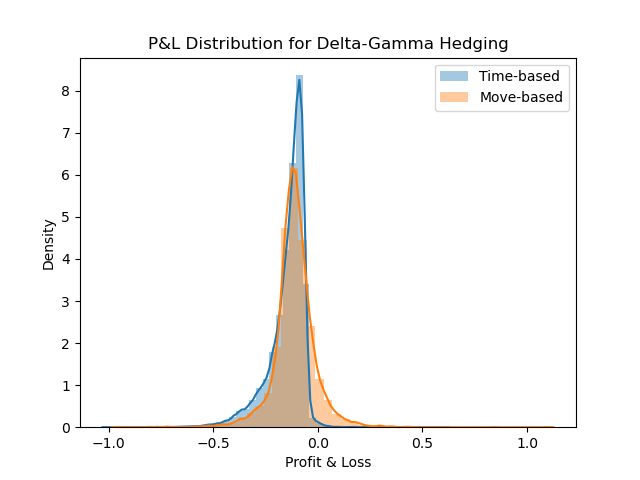
\includegraphics[scale=0.8]{PnLDistributionforDeltaGammaHedging.png}
  \caption[P\&L Distribution for Delta-Gamma Hedging]{P\&L Distribution for Delta-Gamma Hedging}
\end{figure}

\noindent 
Compared to delta-hedging, introducing the gamma parameter did not make both portfolios have a better performance on the mean return but did decrease the variances greatly. Because delta-gamma could detect the underlying asset movement more precisely and return a more concentrated portfolio value.

\subsubsection{Conditional Value at Risk Analysis}
\begin{figure}[H]
  \centering
  \begin{subfigure}{.5\textwidth}
    \centering
    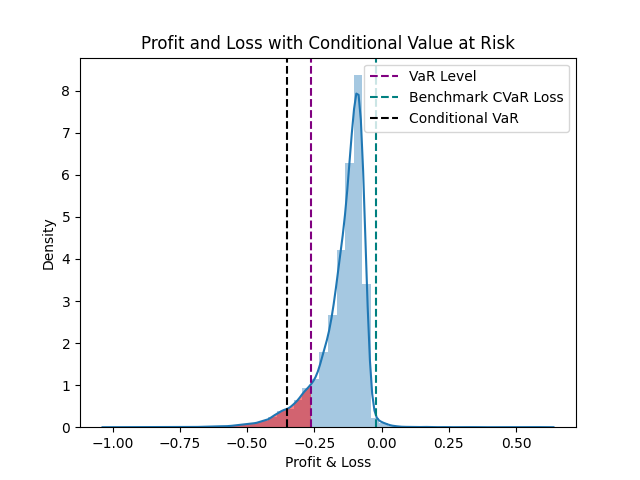
\includegraphics[width=\linewidth]{gamma-var-t.png}
    \caption{Time-based}
  \end{subfigure}%
  \begin{subfigure}{.5\textwidth}
    \centering
    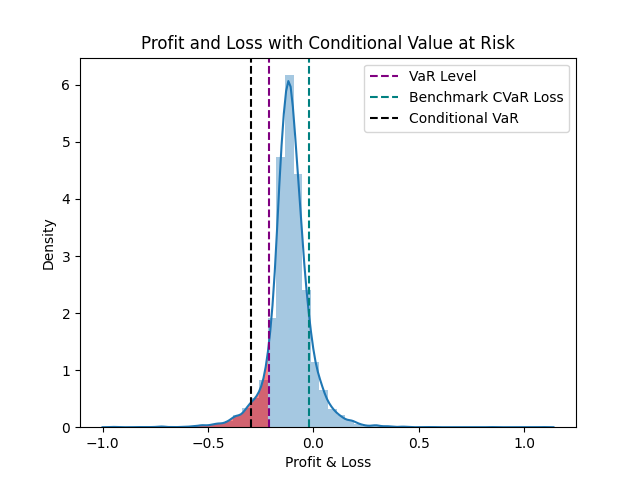
\includegraphics[width=\linewidth]{gamma-var-m.png}
    \caption{Move-based}
  \end{subfigure}%
  \caption{P\&L with Conditional Value at Risk for Delta-Gamma Hedging}
  %\label{fig:test}
\end{figure}

The skewness of the time-based portfolio brings a greater loss than the move-based portfolio: the 90\% VaR is ($-0.26209< -0.20795$) and CVaR is ($-0.35051<-0.29361$). It matches the conclusion discussed above: frequently adjusted portfolio comes with high transaction cost and extreme loss P\&L 
distribution. Therefore it requires a higher option premium to keep the risk value at optimal range. 
\\\\
The following shows the CVaR and adjusted option price observed: 
\begin{enumerate}

  \item The unadjusted option price according to the Delta hedging is 3.7334
  \item CVaR-adjusted option price for Time-based hedging portfolio:

  \begin{itemize}

    \item The VaR for the portfolio at level 0.1 is -0.2621
    \item The CVaR for the portfolio at VaR level 0.1 is  -0.3505
    \item The Adjusted put option price so CVaR at VaR level 0.1 is no smaller than -0.02 is 4.0623

  \end{itemize}

  \item CVaR-adjusted option price for Move-based hedging portfolio:
  
  \begin{itemize}

    \item The VaR for the portfolio at level 0.1 is -0.2079
    \item The CVaR for the portfolio at VaR level 0.1 is -0.2936
    \item The Adjusted put option price so CVaR at VaR level 0.1 is no smaller than -0.02 is 4.0057

  \end{itemize}

\end{enumerate}

\subsection{Delta-hedging with different bandwidth}

From the left plot, the mean number of trade decrease as the bandwidth increase since the larger bandwidth requires less frequent position adjustment. The variance is proportional to the bandwidth. When it applied large bandwidth, if the position hits the boundary and makes an adjustment, 
there will be a significant jump or drop to reach the new position. For the efficient frontier with transaction cost = \$0.005, although the relationship between the standard deviation and mean of P\&L is not quite clear, a general upward trend is there. 
\begin{figure}[H]
  \centering
  \begin{subfigure}{.5\textwidth}
    \centering
    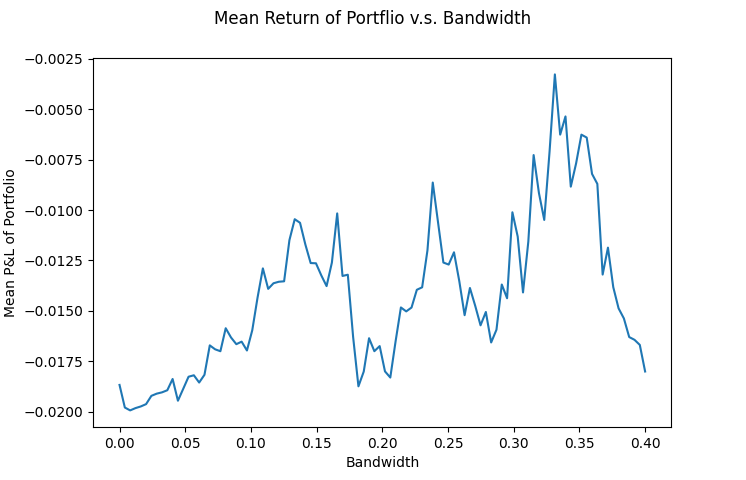
\includegraphics[width=\linewidth]{mean.png}
    \caption{Mean v.s. bandwidth}
  \end{subfigure}%
  \begin{subfigure}{.5\textwidth}
    \centering
    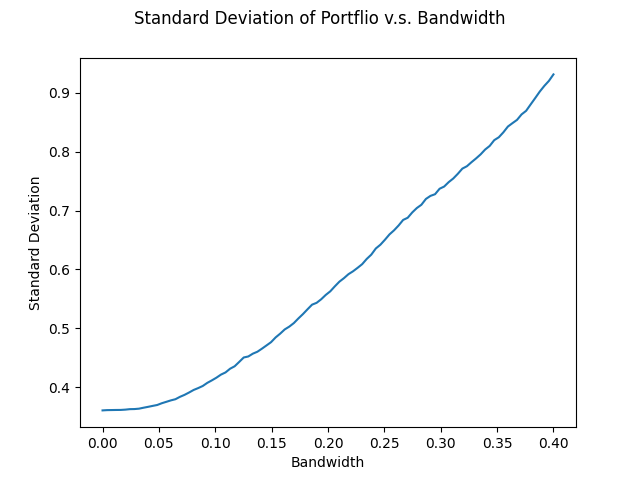
\includegraphics[width=\linewidth]{std.png}
    \caption{Standard Deviation v.s. Bandwidth}
  \end{subfigure}%
  \hfill
  \begin{subfigure}{.5\textwidth}
    \centering
    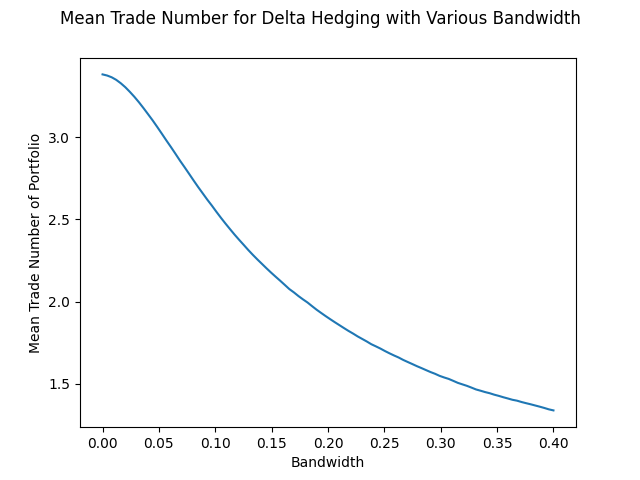
\includegraphics[width=\linewidth]{trade.png}
    \caption{Number of Transactions v.s. Bandwidth}
  \end{subfigure}%
  \caption{Effect of Various Bandwidth for Delta Hedging}
\end{figure}

\noindent
Since the team believe the transaction cost is too small to observe a intuitive plot, the team decided to increase it to \$0.05 (10 times as before) and prove that the portfolio does follow the mean-variance theory. Obviously, the efficient frontier with 0.05 transaction cost follows the mean 
variance theory perfectly. In the situation with having larger the transaction cost, the wider bandwidth portfolio has an advantage in less frequent position adjustment, thus bring a higher variance and lower loss.

\begin{figure}[H]
  \centering
  \begin{subfigure}{.5\textwidth}
    \centering
    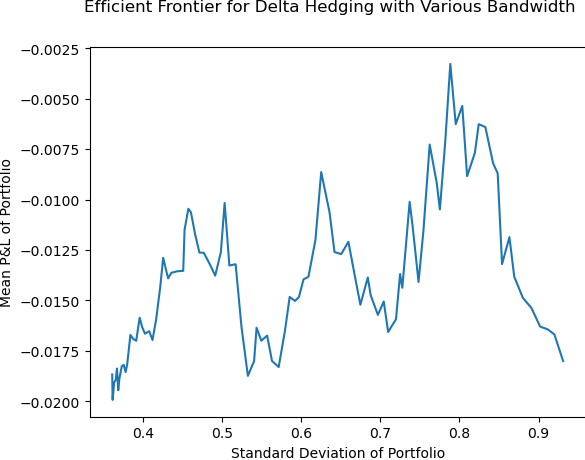
\includegraphics[width=\linewidth]{efficientf1.png}
    \caption{Transaction Cost = \$0.005}
  \end{subfigure}%
  \begin{subfigure}{.5\textwidth}
    \centering
    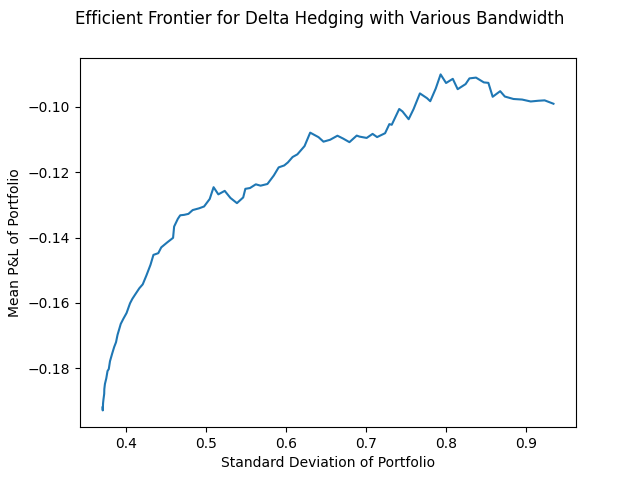
\includegraphics[width=\linewidth]{efficientf2.png}
    \caption{Transaction Cost = \$0.05}
  \end{subfigure}%
  \caption{Mean v.s. Standard Deviation for Various Bandwidth}
\end{figure}

\section{Conclusion}
The report introduces the delta and delta-gamma hedging strategies on two approaches: time-based and move-based. Starting with the mathematical derivation and proof of the theories, then followed by the visualization of the position and portfolio value change under the simulated stock price paths, 
two strategies clearly show how the positions are adjusted and the difference between the portfolio balance. 
\\\\
For the delta hedging strategy, the move-based approach has an advantage in cost efficiency raised from position adjustment, but it brings a higher variance and fatter tail with higher bandwidth. The time-based strategy has a better performance in the portfolio value discrepancy (lower variance) but 
brings a higher transaction cost from more frequent position adjustments. Especially in delta-gamma hedging, after another transaction cost of an option is considered, compared to the move-based approach, it makes the time-based approach costlier and less efficient: a heavily left-skewed P\&L distribution. 
Although the move-based approach still keeps a normal P\&L distribution, the mean of the distribution is negative which means the introduction of another transaction cost does make the two approaches less cost-efficient. But the delta-gamma strategy does make more precise option adjustments and brings smaller 
variances compared to delta hedging. 
\\\\
To solve the “negative mean” problem and manage tolerance of risk, increasing the option price is necessary for the seller to offset part of the loss. Lastly, in the delta hedging, the report observes a proportional relationship between bandwidth and variance. And also, the larger the transaction cost, 
the better shape that efficient frontier has.
\\\\
All the testing and simulations provided in the report create a complete view of understanding two hedging strategies with two different approaches.



\end{document}